
A reverse iterator adapter is an abstraction that reverses the direction of an iterator class. It requires a bidirectional iterator.

\subsubsection{How to do it…}

Most bidirectional containers in the STL include a reverse iterator adapter. Other containers, such as the primitive C-array, do not. Let's look at some examples:

\begin{itemize}
\item 
Let's start with the printc() function we've used throughout this chapter:

\begin{lstlisting}[style=styleCXX]
void printc(const auto & c, const string_view s = "") {
	if(s.size()) cout << format("{}: ", s);
	for(auto e : c) cout << format("{} ", e);
	cout << '\n';
}
\end{lstlisting}

This uses a range-based for loop to print the elements of a container.

\item 
The range-based for loop works even with primitive C-arrays, which have no iterator class. So, our printc() function already works with a C-array:

\begin{lstlisting}[style=styleCXX]
int main() {
	int array[]{ 1, 2, 3, 4, 5 };
	printc(array, "c-array");
}
\end{lstlisting}

We get this output:

\begin{tcblisting}{commandshell={}}
c-array: 1 2 3 4 5
\end{tcblisting}

\item 
We can use the begin() and end() iterator adapters to create normal forward iterators for the C-array:

\begin{lstlisting}[style=styleCXX]
auto it = std::begin(array);
auto end_it = std::end(array);
while (it != end_it) {
	cout << format("{} ", *it++);
}
\end{lstlisting}

Output from the for loop:

\begin{tcblisting}{commandshell={}}
1 2 3 4 5
\end{tcblisting}

\item 
Or we can use the rbegin() and rend() reverse iterator adapters to create reverse iterators for the C-array:

\begin{lstlisting}[style=styleCXX]
auto it = std::rbegin(array);
auto end_it = std::rend(array);
while (it != end_it) {
	cout << format("{} ", *it++);
}
\end{lstlisting}

Now our output is reversed:

\begin{tcblisting}{commandshell={}}
5 4 3 2 1
\end{tcblisting}

\item 
We can even create a modified version of printc() that prints in reverse:

\begin{lstlisting}[style=styleCXX]
void printr(const auto & c, const string_view s = "") {
	if(s.size()) cout << format("{}: ", s);
	auto rbegin = std::rbegin(c);
	auto rend = std::rend(c);
	for(auto it = rbegin; it != rend; ++it) {
		cout << format("{} ", *it);
	}
	cout << '\n';
}
\end{lstlisting}

When we call it with the C-array:

\begin{lstlisting}[style=styleCXX]
printr(array, "rev c-array");
\end{lstlisting}

We get this output:

\begin{tcblisting}{commandshell={}}
rev c-array: 5 4 3 2 1
\end{tcblisting}

\item 
Of course, this works just as well with any bidirectional STL container:

\begin{lstlisting}[style=styleCXX]
vector<int> v{ 1, 2, 3, 4, 5 };
printc(v, "vector");
printr(v, "rev vector");
\end{lstlisting}

Output:

\begin{tcblisting}{commandshell={}}
vector: 1 2 3 4 5
rev vector: 5 4 3 2 1
\end{tcblisting}
\end{itemize}


\subsubsection{How it works…}

A normal iterator class has a begin() iterator that points to the first element, and an end() iterator that points past the last element:

\hspace*{\fill} \\ %插入空行
\begin{center}
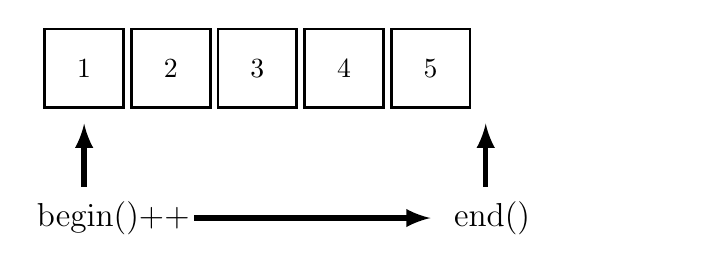
\begin{tikzpicture}
\foreach \x in {1,...,5} {
	\draw[line width=1pt] (1.1*\x,1) rectangle (1.1*\x+1,0) node[pos=.5] {\x};
}

\draw[line width=2pt][-latex] (1.6,-1.0) -- (1.6,-0.2);
\draw[line width=2pt][-latex] (6.7,-1.0) -- (6.7,-0.2);

\node[text width=3cm, font=\large] at (2.5,-1.4) {begin()++};
\node[text width=3cm, font=\large] at (7.8,-1.4) {end()};

\draw[line width=2pt][-latex] (3,-1.4) -- (6.0,-1.4);
\end{tikzpicture}

Figure 4.3 – Forward iterator
\end{center}

You iterate the container by incrementing the begin() iterator with the ++ operator, until it reaches the value of the end() iterator.

A reverse iterator adapter intercepts the iterator interface and turns it around so the begin() iterator points at to the last element, and end() iterator points before the first element. The ++ and -- operators are also inverted:

\hspace*{\fill} \\ %插入空行
\begin{center}
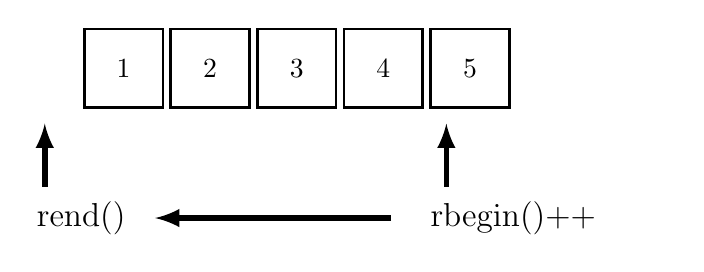
\begin{tikzpicture}
\foreach \x in {1,...,5} {
	\draw[line width=1pt] (1.1*\x,1) rectangle (1.1*\x+1,0) node[pos=.5] {\x};
}

\draw[line width=2pt][-latex] (0.6,-1.0) -- (0.6,-0.2);
\draw[line width=2pt][-latex] (5.7,-1.0) -- (5.7,-0.2);

\node[text width=3cm, font=\large] at (2.0,-1.4) {rend()};
\node[text width=3cm, font=\large] at (7.0,-1.4) {rbegin()++};

\draw[line width=2pt][-latex] (5.0,-1.4) -- (2,-1.4);
\end{tikzpicture}

Figure 4.4 – Reverse iterator adapter
\end{center}


In the reversed iterator, the ++ operator decrements and the -- operator increments.

It's worth noting that most bidirectional STL containers already include a reverse iterator adapter, accessible by member functions rbegin() and rend():

\begin{lstlisting}[style=styleCXX]
vector<int> v;
it = v.rbegin();
it_end = v.rend();
\end{lstlisting}

These iterators will operate in reverse and are suitable for many purposes.
